\documentclass{article}
\usepackage{minted}
\usepackage[utf8]{inputenc}
\usepackage[french]{babel}
\usepackage[T1]{fontenc}
\usepackage{algorithm}
\usepackage{graphicx}
\usepackage{float}
\usepackage{listings}
\usepackage{xcolor}

\title{}
\author{}
\date{}


\setlength{\parindent}{0cm}
\setlength{\parskip}{1ex plus 0.5ex minus 0.2ex}
\newcommand{\hsp}{\hspace{20pt}}
\newcommand{\HRule}{\rule{\linewidth}{0.5mm}}


\title{}
\author{}
\date{}

\makeatletter
\def\BState{\State\hskip-\ALG@thistlm}
\makeatother

\lstset{basicstyle = \ttfamily,columns=fullflexible}


\begin{document}

\begin{titlepage}
  \begin{sffamily}
  \begin{center}

    % Upper part of the page. The '~' is needed because \\
    % only works if a paragraph has started.

    \textsc{\LARGE Polytech Sorbonne}\\[2cm]

    \textsc{\Large EPU-N7-IOB}\\[1.5cm]

    % Title
    \HRule \\[0.4cm]
    { \huge \bfseries Projet final: Space Invader v2\\[0.4cm] }

    \HRule \\[2cm]
    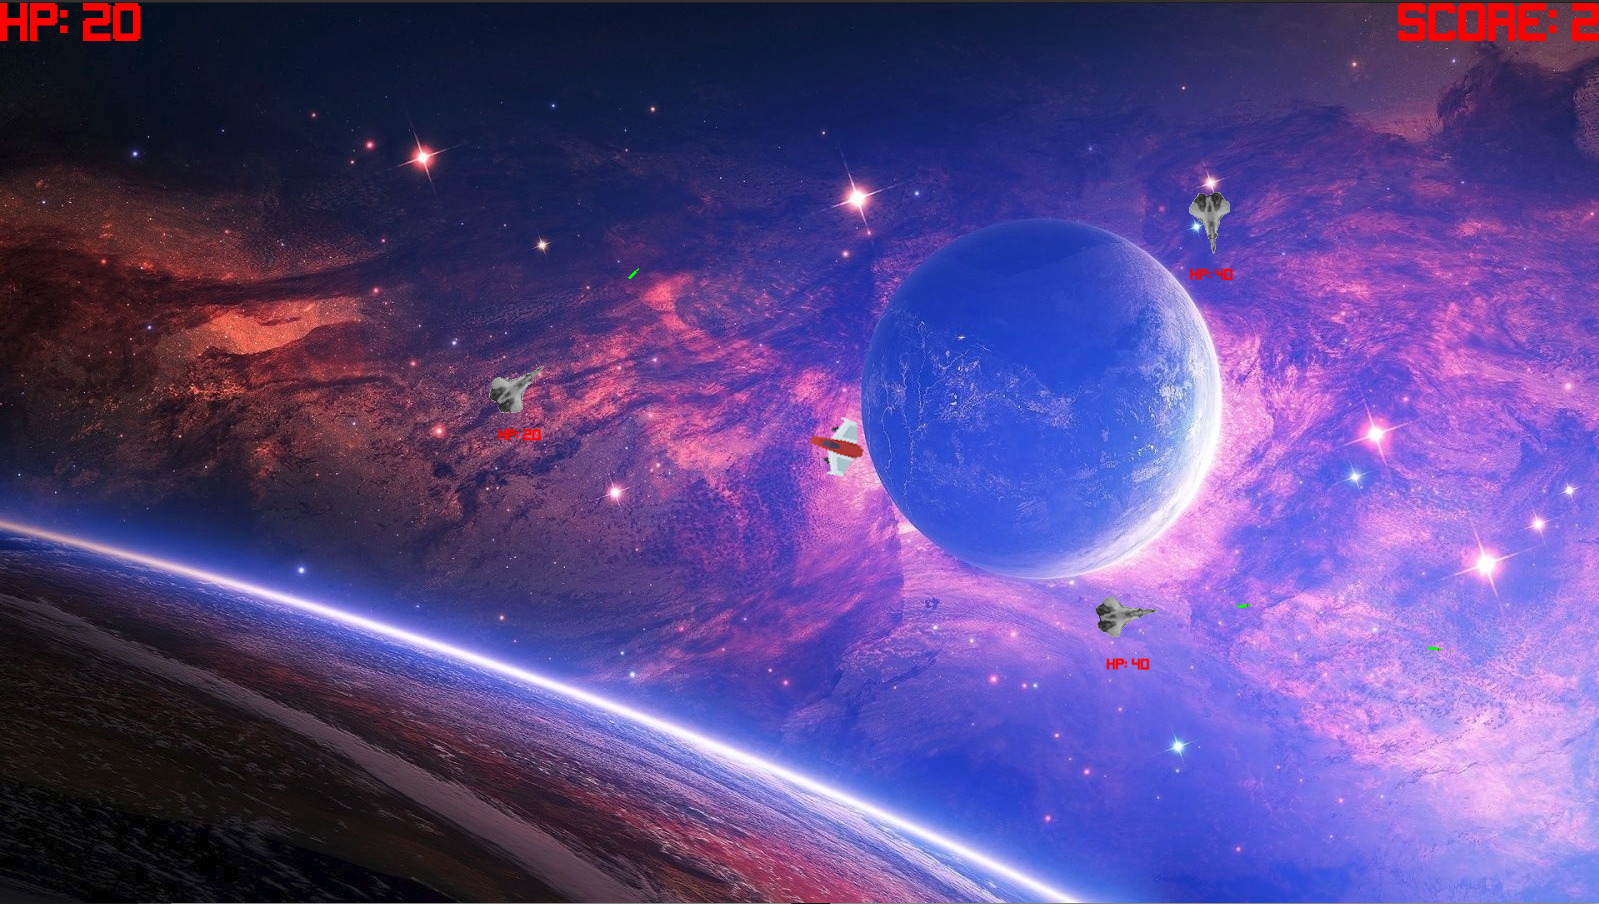
\includegraphics[width=1\textwidth]{assets/img/illustration.png}
    \\[2cm]

    \vfill
    \begin{minipage}{0.4\textwidth}
      \begin{center} \large
        Arthur Guillec\\
      \end{center}
    \end{minipage}
    \vfill

  \end{center}
  \end{sffamily}
\end{titlepage}


\section{Introduction}

Ce rapport traite des principaux aspects du programme et de ses sources.

\section{Le jeu}

L'objectif est similaire à celui du jeu \textbf{Space Invaders}. Le joueur est aux commandes d'un vaisseau spatial et doit se défendre face à une horde d'ennemis déterminés.

Il est possible de se déplacer dans toutes les directions du plan 2D. A chaque fois qu'un vaisseau ennemi est détruit, le score du joueur s'incrémente de un. L'objectif est d'avoir le plus grand score à la fin de la partie, i.e lorsque le vaisseau du joueur n'a plus de vie.

\subsection{Dépendances}

La partie audio et graphique du programme nécessite la bibliothèque \textbf{SFML} (Simple and Fast Multimedia Library). Elle s'installe facilement sur Debian et ses dérivés via la commande:

\begin{lstlisting}[language=bash]
$ sudo apt-get install libsfml-dev
\end{lstlisting}

\subsection{Compilation}

Les sources du programme peuvent être récupérés depuis le dépôt \textbf{GIT} via la commande

\begin{lstlisting}[language=bash]
$ git clone https://github.com/3700240/guillec-projet-cpp
\end{lstlisting}

Un Makefile contenant une règle \textbf{all} et \textbf{clean} est fournit. Une fois la bibliothèque \textbf{SFML} installée, il ne reste donc plus qu'à exécuter la commande

\begin{lstlisting}[language=bash]
$ make
\end{lstlisting}

depuis le répertoire guillec-projet-cpp. puis

\begin{lstlisting}[language=bash]
$ ./game.bin
\end{lstlisting}

pour lancer une partie. Bon jeu!

\section{Les classes}


\subsection{Entity}

La classe \textbf{Entity} est la «super» classe mère dont dérivent toutes les entités, i.e les différents types de vaisseaux et de projectiles.

\begin{minted}{c++} 
class Entity : public sf::Drawable, sf::Transformable
\end{minted}

Elle hérite de sf::Drawable et sf::Transformable. Toutes ces classes filles doivent donc définir la méthode

\begin{minted}{c++} 
virtual void draw(sf::RenderTarget& target, sf::RenderStates states) const;
\end{minted}

Cela permet de les dessiner simplement avec la méthode \textbf{draw} de \textbf{sf::RenderWindow}

\begin{minted}{c++}
// exemple
Entity foo;
...
_win.clear();
_win.draw(foo);
_win.display();
\end{minted}

Chaque entité possède une position, une direction, une vitesse, un rayon (les collisions sont approximées par des cercles).

De plus, elles possèdent un attribut un peu particulier: \textbf{\_isAlive}. Ce dernier décrit si une entité est toujours active. Si ce n'est pas (plus!) le cas, elle sera supprimée à la prochaine itération par des mécanismes similaires à un garbage collector.

\subsection{Character}

La classe \textbf{Character} représente un vaisseau quelconque. Un vaisseau peut être détruit et possède donc une vie. Il est nécessaire d'avoir cette classe entre \textbf{Entity} et \textbf{Player/Ennemy} car les projectiles font des dégâts à tous les vaisseaux, i.e à des \textbf{Character}.

Toutes les classes filles de \textbf{Character} doivent définir la méthode

\begin{minted}{c++}
virtual bool allowedToFire()=0;
\end{minted}

Cette méthode renvoie \textbf{true} si à une itération quelconque de la boucle de jeu, le \textbf{Character} peut tirer une balle.

\subsection{Player}

La classe \textbf{Player} représente le vaisseau du joueur. Un joueur peut tirer une balle toutes les 10 itérations, soit 6 fois par seconde (la logique a lieu à pas constant de 1/60s)

\begin{minted}{c++}
void Player::goTo(sf::Vector2f targetPos)
{
    sf::Vector2f relTargetPos = targetPos-_pos;

    float dot = _dir.x*relTargetPos.x + _dir.y*relTargetPos.y;
    float det = _dir.x*relTargetPos.y - _dir.y*relTargetPos.x;

    float angle = toDegree(std::atan2(det, dot));
    float anglemax = 4.f + (400.f-_speed)/300.f*3.f;
    float rot = (angle>0) ? std::min(angle, anglemax) : std::max(angle, -anglemax); 

    _dir = sf::Vector2f(std::cos(toRadian(rot))*_dir.x-std::sin(toRadian(rot))*_dir.y, 
    	std::sin(toRadian(rot))*_dir.x+std::cos(toRadian(rot))*_dir.y);
    _speed = std::max(std::min(2*magnitude(relTargetPos),400.f) ,100.f);
}
\end{minted}

Sans entrer dans les détails trigonométriques, le joueur change de direction et de vitesse à chaque itération. La nouvelle direction dépend de la position de la souris sur l'écran et ne peut être trop différente de la précédente (la ligne rot=... s'assure que l'angle entre l'ancienne direction et la nouvelle n'est pas trop grand).

La vitesse dépend de la distance entre la souris et le joueur. Plus cette dernière est grande, plus la vitesse l'est aussi.


\subsection{Ennemy}

La classe \textbf{Ennemy} est très similaire à \textbf{Player}. Elle a les mêmes méthodes. La différence est que les actions des \textbf{Ennemy} ne dépendent d'aucune entrée utilisateur. Ce sont donc des I.A. Par exemple, l'action de tir est régit par de l'aléatoire. De plus, la vitesse des ennemis est constante.

\subsection{Bullet}

La classe \textbf{Bullet}.


\subsection{ResourceManager}

Le template \textbf{ResourceManager} a pour rôle de rendre plus simple la manipulation des ressources audios et graphiques. Il s'agit essentiellement d'un \textbf{std::map} aux fonctionnalités étendues. Voici les principales méthodes:

\begin{minted}{c++} 
template <typename Resource, typename Identifier>
class ResourceManager
{
    public:
        void load(Identifier id, const std::string& filename);
        Resource& get(Identifier id);
        const Resource& get(Identifier id) const;
    private:
        void insertResource(Identifier id, std::unique_ptr<Resource> resource);
    private:
        std::map<Identifier, std::unique_ptr<Resource>>	_resourceMap;
};
\end{minted}



Prenons par exemple la classe \textbf{Ennemy} qui permet d'instancier les différents vaisseaux ennemis. Cette classe contient un attribut privé \textbf{\_sprite} de type \textbf{sf::Sprite} utilisé par SFML pour l'affichage. Cet attribut a besoin d'une texture pour être initialisé. Comme il serait coûteux de lire le fichier ennemy.png associé à cette texture à chaque instanciation d'ennemis, on stocke au démarrage du programme la texture dans un \textbf{TextureManager} (i.e un \textbf{ResourceManager<sf::Texture, Textures::ID>} et on y accède via la méthode \textbf{get} et l'identifiant approprié.

\begin{minted}{c++} 
_sprite(textures.get(Textures::Ennemy))
\end{minted}

On définit donc trois types de \textbf{ResourceManager}: un pour chacun des types de ressources manipulées.


\begin{minted}{c++} 
typedef ResourceManager<sf::Texture, Textures::ID> TextureManager;
typedef ResourceManager<sf::Font, Fonts::ID> FontManager;
typedef ResourceManager<sf::SoundBuffer, Sounds::ID> SoundManager;
\end{minted}


\subsection{GameInstance}

La classe \textbf{GameInstance} encapsule l'ensemble des données relatives à une partie.










\section{Boucle de jeu}

Le jeu est articulé autour d'une boucle infinie qui traite les événements (entrées de l'utilisateur), met à jour le jeu (déplacer les entités, gérer les collisions, etc.) puis affiche l'état actuel.

Une des principales difficultés est de faire en sorte que la logique du programme se fasse à fréquence constante tandis que l'affichage se fasse aussi vite que possible.

En effet, si on travaille à pas de temps variable dans la logique de jeu, le risque est que si pour une raison quelconque le programme ralenti, le pas de temps va exploser et nous rencontrerons des problèmes dans les fonctions de collisions.


\begin{minted}{c++} 
void GameInstance::run()
{
    sf::Clock clock;
    sf::Time timeSinceLastUpdate = sf::Time::Zero;
    while(_win.isOpen())
    {
        sf::Time dt = clock.restart();
        timeSinceLastUpdate += dt;
        while(timeSinceLastUpdate > _frameduration)
        {
            timeSinceLastUpdate -= _frameduration;
            manageNewEvents();
            if(_player->isAlive())
                update(_frameduration);
        }
        render();
    }
}
\end{minted}

L'idée dans cette boucle est que la logique est mise à jour uniquement si le temps écoulé depuis la dernière màj est supérieur au pas de temps chosit (ici \textbf{\_frameduration}. L'affichage lui est fait à chaque itération. Ainsi, on obtient bien le comportement souhaité d'un affichage aussi rapide que possible et d'une logique à pas de temps constant.


\section{Conclusion}

\end{document}